% -*- coding: utf-8 -*-
%-------------------------designed by zcf--------------
\documentclass[UTF8,a4paper,10pt]{ctexart}
\usepackage[left=3.17cm, right=3.17cm, top=2.74cm, bottom=2.74cm]{geometry}
\usepackage{amsmath}
\usepackage{graphicx,subfig}
\usepackage{float}
\usepackage{cite}
\usepackage{caption}
\usepackage{enumerate}
\usepackage{booktabs} %表格
\usepackage{multirow}
\newcommand{\tabincell}[2]{\begin{tabular}{@{}#1@{}}#2\end{tabular}}  %表格强制换行
%-------------------------字体设置--------------
\usepackage{times} 
\newcommand{\yihao}{\fontsize{26pt}{36pt}\selectfont}           % 一号, 1.4 倍行距
\newcommand{\erhao}{\fontsize{22pt}{28pt}\selectfont}          % 二号, 1.25倍行距
\newcommand{\xiaoer}{\fontsize{18pt}{18pt}\selectfont}          % 小二, 单倍行距
\newcommand{\sanhao}{\fontsize{16pt}{24pt}\selectfont}  %三号字
\newcommand{\xiaosan}{\fontsize{15pt}{22pt}\selectfont}        % 小三, 1.5倍行距
\newcommand{\sihao}{\fontsize{14pt}{21pt}\selectfont}            % 四号, 1.5 倍行距
\newcommand{\banxiaosi}{\fontsize{13pt}{19.5pt}\selectfont}    % 半小四, 1.5倍行距
\newcommand{\xiaosi}{\fontsize{12pt}{18pt}\selectfont}            % 小四, 1.5倍行距
\newcommand{\dawuhao}{\fontsize{11pt}{11pt}\selectfont}       % 大五号, 单倍行距
\newcommand{\wuhao}{\fontsize{10.5pt}{15.75pt}\selectfont}    % 五号, 单倍行距
%-------------------------章节名----------------
\usepackage{ctexcap} 
\CTEXsetup[name={,、},number={ \chinese{section}}]{section}
\CTEXsetup[name={(,)},number={\chinese{subsection}}]{subsection}
\CTEXsetup[name={,.},number={\arabic{subsubsection}}]{subsubsection}
%-------------------------页眉页脚--------------
\usepackage{fancyhdr}
\pagestyle{fancy}
\lhead{\kaishu \leftmark}
% \chead{}
\rhead{\kaishu 网络安全技术实验报告}%加粗\bfseries 
\lfoot{}
\cfoot{\thepage}
\rfoot{}
\renewcommand{\headrulewidth}{0.1pt}  
\renewcommand{\footrulewidth}{0pt}%去掉横线
\newcommand{\HRule}{\rule{\linewidth}{0.5mm}}%标题横线
\newcommand{\HRulegrossa}{\rule{\linewidth}{1.2mm}}
%-----------------------伪代码------------------
\usepackage{algorithm}  
\usepackage{algorithmicx}  
\usepackage{algpseudocode}  
\floatname{algorithm}{Algorithm}  
\renewcommand{\algorithmicrequire}{\textbf{Input:}}  
\renewcommand{\algorithmicensure}{\textbf{Output:}} 
\usepackage{lipsum}  
\makeatletter
\newenvironment{breakablealgorithm}
  {% \begin{breakablealgorithm}
  \begin{center}
     \refstepcounter{algorithm}% New algorithm
     \hrule height.8pt depth0pt \kern2pt% \@fs@pre for \@fs@ruled
     \renewcommand{\caption}[2][\relax]{% Make a new \caption
      {\raggedright\textbf{\ALG@name~\thealgorithm} ##2\par}%
      \ifx\relax##1\relax % #1 is \relax
         \addcontentsline{loa}{algorithm}{\protect\numberline{\thealgorithm}##2}%
      \else % #1 is not \relax
         \addcontentsline{loa}{algorithm}{\protect\numberline{\thealgorithm}##1}%
      \fi
      \kern2pt\hrule\kern2pt
     }
  }{% \end{breakablealgorithm}
     \kern2pt\hrule\relax% \@fs@post for \@fs@ruled
  \end{center}
  }
\makeatother
%------------------------代码-------------------
\usepackage{xcolor} 
\usepackage{listings} 
\usepackage{fontspec}
\newfontfamily\menlo{Menlo}
\setmonofont[Mapping={}]{Monaco} 
\definecolor{mygreen}{rgb}{0,0.6,0}
\definecolor{mygray}{rgb}{0.5,0.5,0.5}
\definecolor{mymauve}{rgb}{0.58,0,0.82}
\lstset{ %
backgroundcolor=\color{white},   % choose the background color
basicstyle=\footnotesize\ttfamily,        % size of fonts used for the code
columns=fullflexible,
breaklines=true,                 % automatic line breaking only at whitespace
captionpos=b,                    % sets the caption-position to bottom
tabsize=4,
commentstyle=\color{mygreen},    % comment style
escapeinside={\%*}{*)},          % if you want to add LaTeX within your code
keywordstyle=\color{blue},       % keyword style
stringstyle=\color{mymauve}\ttfamily,     % string literal style
frame=single,
rulesepcolor=\color{red!20!green!20!blue!20},
numbers=left,
 numberstyle=\tiny\menlo
% identifierstyle=\color{red},
% language=c++,
}
%------------超链接----------
\usepackage[colorlinks,linkcolor=black,anchorcolor=blue]{hyperref}
%------------------------TODO-------------------
\usepackage{enumitem,amssymb}
\newlist{todolist}{itemize}{2}
\setlist[todolist]{label=$\square$}
% for check symbol 
\usepackage{pifont}
\newcommand{\cmark}{\ding{51}}%
\newcommand{\xmark}{\ding{55}}%
\newcommand{\done}{\rlap{$\square$}{\raisebox{2pt}{\large\hspace{1pt}\cmark}}\hspace{-2.5pt}}
\newcommand{\wontfix}{\rlap{$\square$}{\large\hspace{1pt}\xmark}}
%------------------------水印-------------------
\usepackage{tikz}
\usepackage{xcolor}
\usepackage{eso-pic}

\newcommand{\watermark}[3]{\AddToShipoutPictureBG{
\parbox[b][\paperheight]{\paperwidth}{
\vfill%
\centering%
\tikz[remember picture, overlay]%
  \node [rotate = #1, scale = #2] at (current page.center)%
    {\textcolor{gray!80!cyan!30!magenta!30}{#3}};
\vfill}}}



%———————————————————————————————————————————正文———————————————————————————————————————————————
%----------------------------------------------
\begin{document}
\begin{titlepage}
    \begin{center}
    
\includegraphics[width=0.8\textwidth]{NKU.png}\\[1cm]    
    \textsc{\Huge \kaishu{\textbf{南\ \ \ \ \ \ 开\ \ \ \ \ \ 大\ \ \ \ \ \ 学}} }\\[0.9cm]
    \textsc{\huge \kaishu{\textbf{计\ \ 算\ \ 机\ \ 学\ \ 院}}}\\[0.5cm]
    \textsc{\Large \textbf{网络安全技术作业报告}}\\[0.8cm]
    \HRule \\[0.9cm]
    { \LARGE \bfseries 基于RSA算法自动分配密钥的加密聊天程序}\\[0.4cm]
    \HRule \\[2.0cm]
    \centering
    \textsc{\LARGE \kaishu{朱浩泽\ 1911530}}\\[0.5cm]
    \textsc{\LARGE \kaishu{年级\ :\ 2019级}}\\[0.5cm]
    \textsc{\LARGE \kaishu{专业\ :\ 计算机科学与技术}}\\[0.5cm]
    \textsc{\LARGE \kaishu{班级\ :\ 计算机科学与技术2班}}\\[0.5cm]
    \vfill
    {\Large \today}
    \end{center}
\end{titlepage}
% -------------摘------要--------------
\newpage
\thispagestyle{empty}
% ----------------------------------------------------------------
\tableofcontents
% ----------------------------------------------------------------
\newpage
\watermark{60}{10}{NKU}
\setcounter{page}{1}
\section{实验目的}
\begin{enumerate}
  \item 加深对RSA 算法基本工作原理的理解。
  \item 掌握基于RSA 算法的保密通信系统的基本设计方法。
  \item 掌握在Linux 操作系统实现RSA 算法的基本编程方法。
  \item 了解Linux 操作系统异步IO 接口的基本工作原理。
\end{enumerate}
\section{实验内容}
\begin{enumerate}
  \item 要求在Linux 操作系统中完成基于RSA 算法的自动分配密钥加密聊天程序的编写。
  \item 应用程序保持第三章“基于DES 加密的TCP 通信”中示例程序的全部功能,并在此基础上进行扩展,实现密钥自动生成,并基于RSA 算法进行密钥共享。
  \item 要求程序实现全双工通信,并且加密过程对用户完全透明。
\end{enumerate}
\section{实验步骤及实验结果}
\subsection{实验环境}
\noindent macOS 12.3(基于 unix), C++11, Cmake\
\subsection{代码结构}
\noindent CDesOperate.h CDesOperate.cpp 封装了DES 加密解密的CDesOperate 类。\\
CRsaOperate.h CRsaOperate.cpp 封装了RSA 加密解密的CRsaOperate 类。\\
head.h main.cpp 服务器和客户端的处理函数。\\
\begin{center}
  \includegraphics*[]{1.jpg}
  \includegraphics*[]{2.jpg}
  \includegraphics*[]{3.jpg}
  \includegraphics*[]{4.jpg}
\end{center}

\subsection{代码实现}
\subsubsection{封装DES 加密解密算法的类}
CDesOperate 类较实验一没有发生变化,后文对此类不加赘述。
\subsubsection{封装RSA 加密解密算法的类,并检验其正确性。}
建立两个数据结构,存储 RSA 公私钥对的全部数据
\begin{lstlisting}[language = c++]
struct PublicKey {
    __int64 nE;
    __int64 nN;
};

struct RSAKeyPair {
    __int64 publicKey_e;
    __int64 secretKey_d;
    __int64 n;
};
\end{lstlisting}
m\_cParament,该变量是存储RSA 的基本参数,定义如下:
\begin{lstlisting}[language = C++]
struct RsaParam{
    __int64 e;
    __int64 n;
    __int64 d;
    __int64 f;
    __int64 p;
    __int64 q;
    __int64 s;
};  
\end{lstlisting}
编写RSA.h 和RSA.cpp 两个文件,在RSA.h 文件中进行函数与类的声明,
在RSA.cpp 文件中进行定义。\\
CRsaOperate 类中的内容
\begin{itemize}
  \item MulMod()\\ 
  模乘运算即计算两个数的乘积然后取模
  \item PowMod()\\
  快速模幂运算
  \item MillerRabin()\\
  MillerRabin 素数测试算法
  \item RandomPrime() \\ 
  质数生成函数RandomPrime
  \item Gcd()\\ 
  求最大公约数
  \item Euler()\\
  欧拉函数:返回小于n 且与n 互质的正整数个数
  \item GetPublicKey()\\
  获取公钥
  \item NewRsaKeyPair()\\
  生成RSA 公私钥对
  \item Encry()\\
  加密函数
  \item Decry()\\
  解密函数
\end{itemize}

\begin{lstlisting}[language = c++]
class CRsaOperate {
public:
    RsaParam m_cParament;  
    CRsaOperate(); 
    static inline __int64 MulMod(__int64 a, unsigned long b, unsigned long n);
    static __int64 PowMod(__int64 base, __int64 pow, __int64 n);
    static long RabinMillerKnl(__int64 &n);
    static long RabinMiller(__int64 &n, long loop);
    static __int64 RandPrime(char bit);
    static __int64 Gcd(__int64 &p, __int64 &q);
    static __int64 Euclid(__int64 e, __int64 t_n);
    static __int64 Encry(unsigned short nScore, PublicKey &cKey);
    unsigned short Decry(__int64 nScore);
    PublicKey GetPublicKey();
};
\end{lstlisting}

\begin{itemize}
  \item 模乘运算\\ 
  模乘运算即计算两个数的乘积然后取模
  \begin{lstlisting}[language = c++]
inline __int64 CRsaOperate::MulMod(__int64 a, unsigned long b, unsigned long n) {
    return (a % n) * (b % n) % n;
}
\end{lstlisting}
  \item 快速模幂运算\\
  利用快速幂算法进行快速模幂计算,可以在保证数据准确的情况下,快速得到高次幂模运算后的结果。
  \begin{lstlisting}[language = c++]
__int64 CRsaOperate::PowMod(__int64 base, __int64 pow, __int64 n) {
    __int64 a = base, b = pow, c = 1;
    while(b){
        while(!(b & 1)){
            b >>= 1;
            a = MulMod(a, a, n);
        }
        b--;
        c = MulMod(a, c, n);
    }
    return c;
}
  \end{lstlisting}
  \item MillerRabin 素数测试算法\\
  概率算法:MillerRabin 素数测试算法\\
  缺省参数loop 为默认重复测试参数为100\\
  Rabin-Miller 算法具有较低的时间复杂度,但是无法保证所得结果一定是正确的,而是以一定的概率得到一个素数,所以需要设定一个安全参数来保证Rabin-Miller 算法以高概率得到一个素数。
  \begin{lstlisting}[language = c++]
long CRsaOperate::RabinMillerKnl(__int64 &n) {
    __int64 a, q, k, v;
    q = n - 1;
    k = 0;
    while(!(q & 1)) {
        ++k;
        q >>= 1;
    }
    a = 2 + rand() % (n - 3);
    v = PowMod(a, q, n);
    if(v == 1) {
        return 1;
    }
    for(int j = 0; j < k; j++) {
        unsigned int z = 1;
        for(int w = 0; w < j; w++) {
            z *= 2;
        }
        if(PowMod(a, z*q, n) == n - 1)
            return 1;
    }
    return 0;
}


long CRsaOperate::RabinMiller(__int64 &n, long loop=100) {
    for(long i = 0; i < loop ; i++){
        if(!RabinMillerKnl(n)){
            return 0;
        }
    }
    return 1;
}
  \end{lstlisting}
  \item 质数生成函数RandomPrime\\ 
  保证最高位是1,再加上一个随机数,保证最低位是1,即保证是奇数,进行拉宾-米勒测试30次,全部通过认为是质数
  \begin{lstlisting}[language = C++]
__int64 CRsaOperate::RandPrime(char bit) {
    __int64 base;
    do{
        base = (unsigned long)1 << (bit - 1);
        base += rand() % (base);
        base |= 1;
    }
    while(!RabinMiller(base, 30));
    return base;
}
  \end{lstlisting}
  \item 求最大公约数\\
  两数相等,最大公约数就是本身;辗转相除法,gcd(a,b)=gcd(b, a-qb)。求解方式这个方程组的方法是拓展的欧几里得算法。
  \begin{lstlisting}[language = C++]
__int64 CRsaOperate::Gcd(__int64 &p, __int64 &q) {
    unsigned long long a = p > q ? p : q;
    unsigned long long b = p < q ? p : q;
    unsigned long long t;
    if( p == q ){
        return p;
    }else{
        while(b){
            a = a % b;
            t = a;
            a = b;
            b = t;
        }
        return a;
    }
}
  \end{lstlisting}
  \item 欧拉函数:返回小于n 且与n 互质的正整数个数
  \begin{lstlisting}[language = C++]
__int64 CRsaOperate::Euclid(__int64 e, __int64 t_n) { 
    unsigned long long Max = 0xffffffffffffffff - t_n;
    unsigned long long i = 1;
    while(1){
        if(((i*t_n)+1)%e == 0){
            return ((i*t_n)+1)/e;
        }
        i++;
        unsigned long long Tmp = (i+1)*t_n;
        if(Tmp > Max){
            return 0;
        }
    }
    return 0;
}    
  \end{lstlisting}
  \item 公私钥对生成\\
  除了加解密函数外,另外一个重要的内容是RSA 大素数生成问题。在CRSASection 类中RsaGetParam 函数是用来生成RSA 所有必要的参数,其中主要内容都是生成两个大素数。
  \begin{lstlisting}[language = C++]
RsaParam RsaGetParam() {
    RsaParam Rsa = { 0 };
    unsigned long long t;
    Rsa.p = CRsaOperate::RandPrime(16);
    Rsa.q = CRsaOperate::RandPrime(16);
    Rsa.n = Rsa.p * Rsa.q;
    Rsa.f = (Rsa.p - 1) * (Rsa.q - 1);
    do {
        Rsa.e = rand() % Rsa.f;
        Rsa.e |= 1;
    }
    while(CRsaOperate::Gcd(Rsa.e, Rsa.f) != 1);
    Rsa.d = CRsaOperate::Euclid(Rsa.e, Rsa.f);
    Rsa.s = 0;
    t = Rsa.n >> 1;
    while(t) {
        Rsa.s++;
        t >>= 1;
    }
    return Rsa;
}
  \end{lstlisting}
  \item 获取公钥对
  \begin{lstlisting}[language = C++]
PublicKey CRsaOperate::GetPublicKey() {
    PublicKey cTmp;
    cTmp.nE = this -> m_cParament.e;
    cTmp.nN = this -> m_cParament.n;
    return cTmp;
}
  \end{lstlisting}
  \item RSA解密函数
  \begin{lstlisting}[language = C++]
unsigned short CRsaOperate::Decry(__int64 nScore) {
    unsigned long long nRes = PowMod(nScore, m_cParament.d, m_cParament.n);
    unsigned short *pRes = (unsigned short *)&(nRes);
    if(pRes[1] != 0 || pRes[3] != 0 || pRes[2] != 0) {
        return 0;
    }
    else {
        return pRes[0];
    }
}
  \end{lstlisting}
\end{itemize}
\subsubsection{通讯部分}
服务端将公钥发送给希望与其通话的客户端,然后客户端就可以通过公钥加密生成的DES 密钥发送给服务端,服务端收到消息后利用自己的私钥进行解密便成功与客户端得到了相同的会话密钥。
\begin{itemize}
  \item \textbf{客户端函数}\\ 
  与服务器建立连接后,客户端接收到服务器发送的RSA 公钥对后,随机生成DES 密钥并用公钥对加密发送给服务器;此后,用DES 密钥进行聊天。
  \begin{lstlisting}[language = C++]
else {
    std::cout << "Please input the server address:" << std::endl;
    char strIPAddr[16];
    std::cin >> strIPAddr;
    int nConnectSocket, nLength;
    struct sockaddr_in sDestAddr;
    if((nConnectSocket = socket(AF_INET,SOCK_STREAM, 0)) < 0) {
        perror("Socket");
        exit(errno);
    }
    int SEVERPORT = 6000;

    sDestAddr.sin_family = AF_INET;
    sDestAddr.sin_port = htons(SEVERPORT);
    sDestAddr.sin_addr.s_addr = inet_addr(strIPAddr);
    if(connect(nConnectSocket, (struct sockaddr *) &sDestAddr, sizeof(sDestAddr)) != 0) {
        perror("Connect");
        exit(errno);
    }
    else {
        printf("Connect Success! \n");
        char *strDesKey = new char [8];
        GerenateDesKey(strDesKey);
        printf("Create DES key success\n");
        PublicKey cRsaPublicKey;
        if(sizeof(cRsaPublicKey) == TotalRecv(nConnectSocket,(char *)&cRsaPublicKey, sizeof(cRsaPublicKey),0)) {
            printf("Successful get the RSA public Key\n");
        }
        else {
            perror("Get RSA public key ");
            exit(0);
        }
        unsigned long long nEncryptDesKey[4];
        unsigned short *pDesKey = (unsigned short *)strDesKey;
        for(int i = 0; i < 4; i++) {
            nEncryptDesKey[i] = CRsaOperate::Encry(pDesKey[i],cRsaPublicKey);
        }
        if(sizeof(unsigned long long)*4 != send(nConnectSocket, (char *)nEncryptDesKey,sizeof(unsigned long long)*4, 0)) {
            perror("Send DES key Error");
            exit(0);
        }
        else {
            printf("Successful send the encrypted DES Key\n");
        }
        printf("Begin to chat...\n");
        SecretChat(nConnectSocket,strIPAddr,strDesKey);
    }
    close(nConnectSocket);
}
  \end{lstlisting}
  \item \textbf{服务器函数} \\
  与客户端建立连接后,生成RSA 公私钥对,并将公钥对发送给客户端,然后接收客户端发来的加过密的DES 密钥,用自己的私钥对解密;此后,用DES 密钥进行通信。
  \begin{lstlisting}[language = C++]
  if(temp == 's') {
      int nListenSocket,nAcceptSocket;
      struct sockaddr_in sLocalAddr, sRemoteAddr;
      bzero(&sLocalAddr, sizeof(sLocalAddr));
      sLocalAddr.sin_family = PF_INET;
      sLocalAddr.sin_port = htons(6000);
      sLocalAddr.sin_addr.s_addr = INADDR_ANY;
      if ((nListenSocket = socket(PF_INET, SOCK_STREAM, 0)) == -1) {
          perror("socket");
          exit(1);
      }
      if(bind(nListenSocket, (struct sockaddr *) &sLocalAddr, sizeof(struct sockaddr)) == -1) {
          perror("bind");
          exit(1);
      }
      if(listen(nListenSocket, 5) == -1) {
          perror("listen");
          exit(1);
      }
      printf("Listening...\n");
      socklen_t nLength = 0;
      nAcceptSocket = accept(nListenSocket, (struct sockaddr*)&sRemoteAddr, &nLength);
      close(nListenSocket);
      printf("server: got connection from %s, port %d, socket %d\n",inet_ntoa(sRemoteAddr.sin_addr), ntohs(sRemoteAddr.sin_port), nAcceptSocket);
      
      //negotiate key
      PublicKey cRsaPublicKey;
      CRsaOperate CRsaOperate;
      //CRsaOperate.show_par();
      cRsaPublicKey = CRsaOperate.GetPublicKey();
      if(send(nAcceptSocket, (char *)(&cRsaPublicKey), sizeof(cRsaPublicKey), 0) != sizeof(cRsaPublicKey)){
          perror("send");
          exit(0);
      }else{
          printf("successful send the RSA public key. \n");
      }
      unsigned long long nEncryptDesKey[4];
      char *strDesKey = new char[8];
      if(4*sizeof(unsigned long long) != TotalRecv(nAcceptSocket,(char *)nEncryptDesKey, 4*sizeof(unsigned long long),0)) {
          perror("TotalRecv DES key error");
          exit(0);
      }
      else {
          printf("successful get the DES key\n");
          unsigned short * pDesKey = (unsigned short *)strDesKey;
          for(int i = 0;i < 4; i++) {
              pDesKey[i] = CRsaOperate.Decry(nEncryptDesKey[i]);
              //cout << pDesKey[i] << endl;
          }
      }
      
      printf("Begin to chat...\n");
      SecretChat(nAcceptSocket,inet_ntoa(sRemoteAddr.sin_addr),strDesKey);
      close(nAcceptSocket);
  }
  \end{lstlisting}
  \item \textbf{SecretChat函数} \\ 
  用select 模型重写通信函数。传统的网络通信I/O 是阻塞I/O 或者非阻塞I/O,阻塞I/O 会使得进程必须暂停下来等到I/O 事件的完全,非阻塞I/O 则需要进行轮询,大量消耗CPU 资源。因此出现了一种新的网络I/O 模型——select 模型。select 模型的基本特点是可以一次性监听多个I/O 请求,虽然本质上还是阻塞I/O,但是由于其具备了一次性处理多个I/O 的能力,所以可以大大加大网络I/O 的效率。利用select 模型重写SecretChat 函数,首先初始化文件列表、等待时间、返回值。然后开始一个循环进行监听,每次监听之前先对于select 模型进行询问,查看其中完成的I/O 请求,以便多次处理。然后对于sock 套接字和标准输入的文件描述符进行监听。对于sock 套接字的监听。一旦存在sock 套接字的请求便进行处理。对于标准输入的处理。一旦用户进行输入,便进行处理。
  \begin{lstlisting}[language = C++]
void SecretChat(int nSock, char *pRemoteName, char *pKey) {

    std::cout << pRemoteName << std::endl;
    CDesOperate cDes;
    std::cout << pKey << std::endl;
    int klength = strlen(pKey);
    if(klength != 8){
        printf("%s\n",pKey);
        printf("Key length error\n");
        return;
    }

    //select model
    fd_set cHandleSet;
    struct timeval tv;
    int nRet;
    while(1){
        FD_ZERO(&cHandleSet);
        FD_SET(nSock, &cHandleSet);
        FD_SET(0, &cHandleSet);
        tv.tv_sec = 1;
        tv.tv_usec = 0;
        nRet = select(nSock>0? nSock+ 1:1, &cHandleSet, NULL, NULL, &tv);
        if(nRet < 0){
            printf("Select error!\n");
            break;
        }
        if(nRet == 0){
            continue;
        }
        if(FD_ISSET(nSock,&cHandleSet)){
            bzero(&strSocketBuffer, BUFFERSIZE);
            int nLength = 0;
            nLength = TotalRecv(nSock, strSocketBuffer,BUFFERSIZE,0);
            if(nLength !=BUFFERSIZE) break;
            else{
                int nLen = BUFFERSIZE;
                cDes.Decry(strSocketBuffer,BUFFERSIZE,strDecryBuffer,nLen,pKey,8);
                strDecryBuffer[BUFFERSIZE-1]=0;
                if(strDecryBuffer[0]!=0&&strDecryBuffer[0]!='\n'){
                    printf("Receive message form <%s>: %s",pRemoteName,strDecryBuffer);
                    if(0==memcmp("quit",strDecryBuffer,4)){
                        printf("Quit!\n");
                        break;
                    }
                }
            }
        }
        if(FD_ISSET(0,&cHandleSet)){
            bzero(&strStdinBuffer, BUFFERSIZE);
            while(strStdinBuffer[0]==0){
                if (fgets(strStdinBuffer, BUFFERSIZE, stdin) == NULL){
                    continue;
                }
            }
            int nLen = BUFFERSIZE;
            cDes.Encry(strStdinBuffer,BUFFERSIZE,strEncryBuffer,nLen,pKey,8);
            if(send(nSock, strEncryBuffer, BUFFERSIZE,0)!=BUFFERSIZE){
                perror("send");
            }else{
                if(0==memcmp("quit",strStdinBuffer,4)){
                    printf("Quit!\n");
                    break;
                }
            }
        }
    }
}
  \end{lstlisting}
  \item \textbf{GerenateDesKey函数} \\
  随机生成DES 密钥。
  \begin{lstlisting}[language = C++]
void GerenateDesKey(char* x){
    int i;
    srand(time(NULL));
    for (i = 0; i < 8; i++)
    {
        switch ((rand() % 3))
        {
        case 1:
            x[i] = 'A' + rand() % 26;
            break;
        case 2:
            x[i] = 'a' + rand() % 26;
            break;
        default:
            x[i] = '0' + rand() % 10;
            break;
        }
    }
    x[i] = '\0';
}
  \end{lstlisting}
\end{itemize}




\section{实验结果}
客户端上线,连接成功
\begin{center}
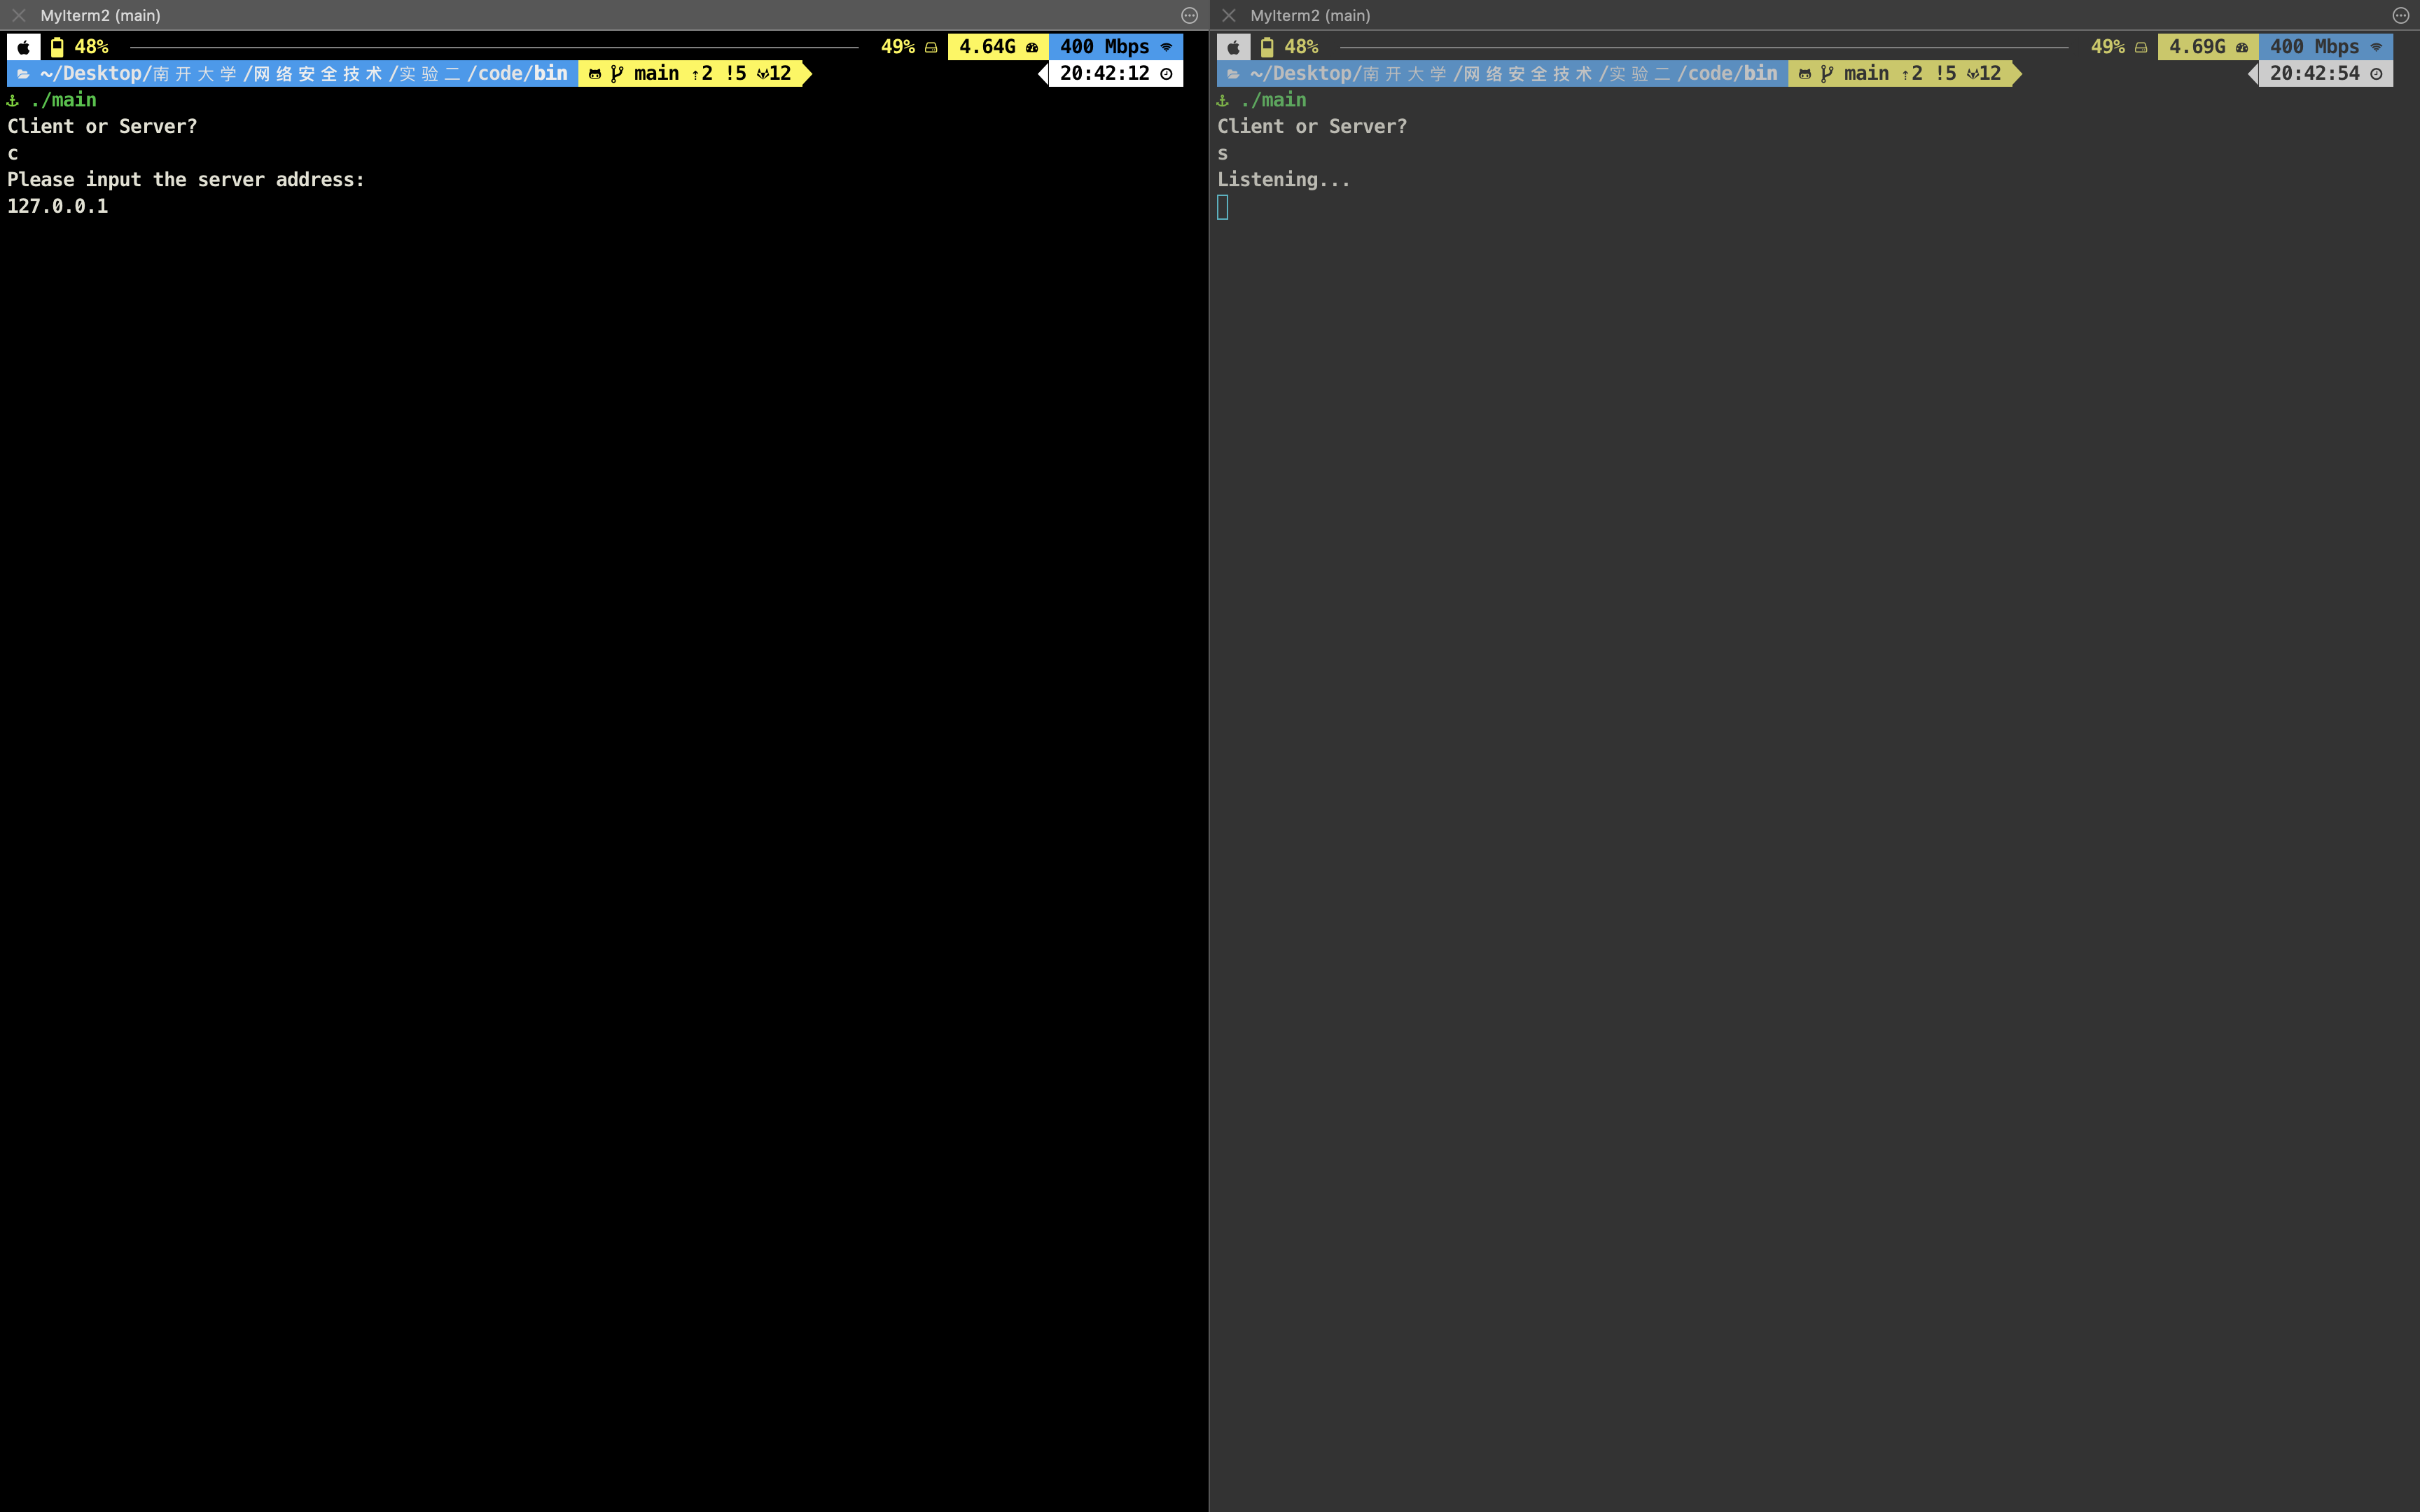
\includegraphics[scale = 0.23]{1.png}
\end{center}
客户端生成DES密钥并传输到服务器,服务器解密成功
\begin{center}
  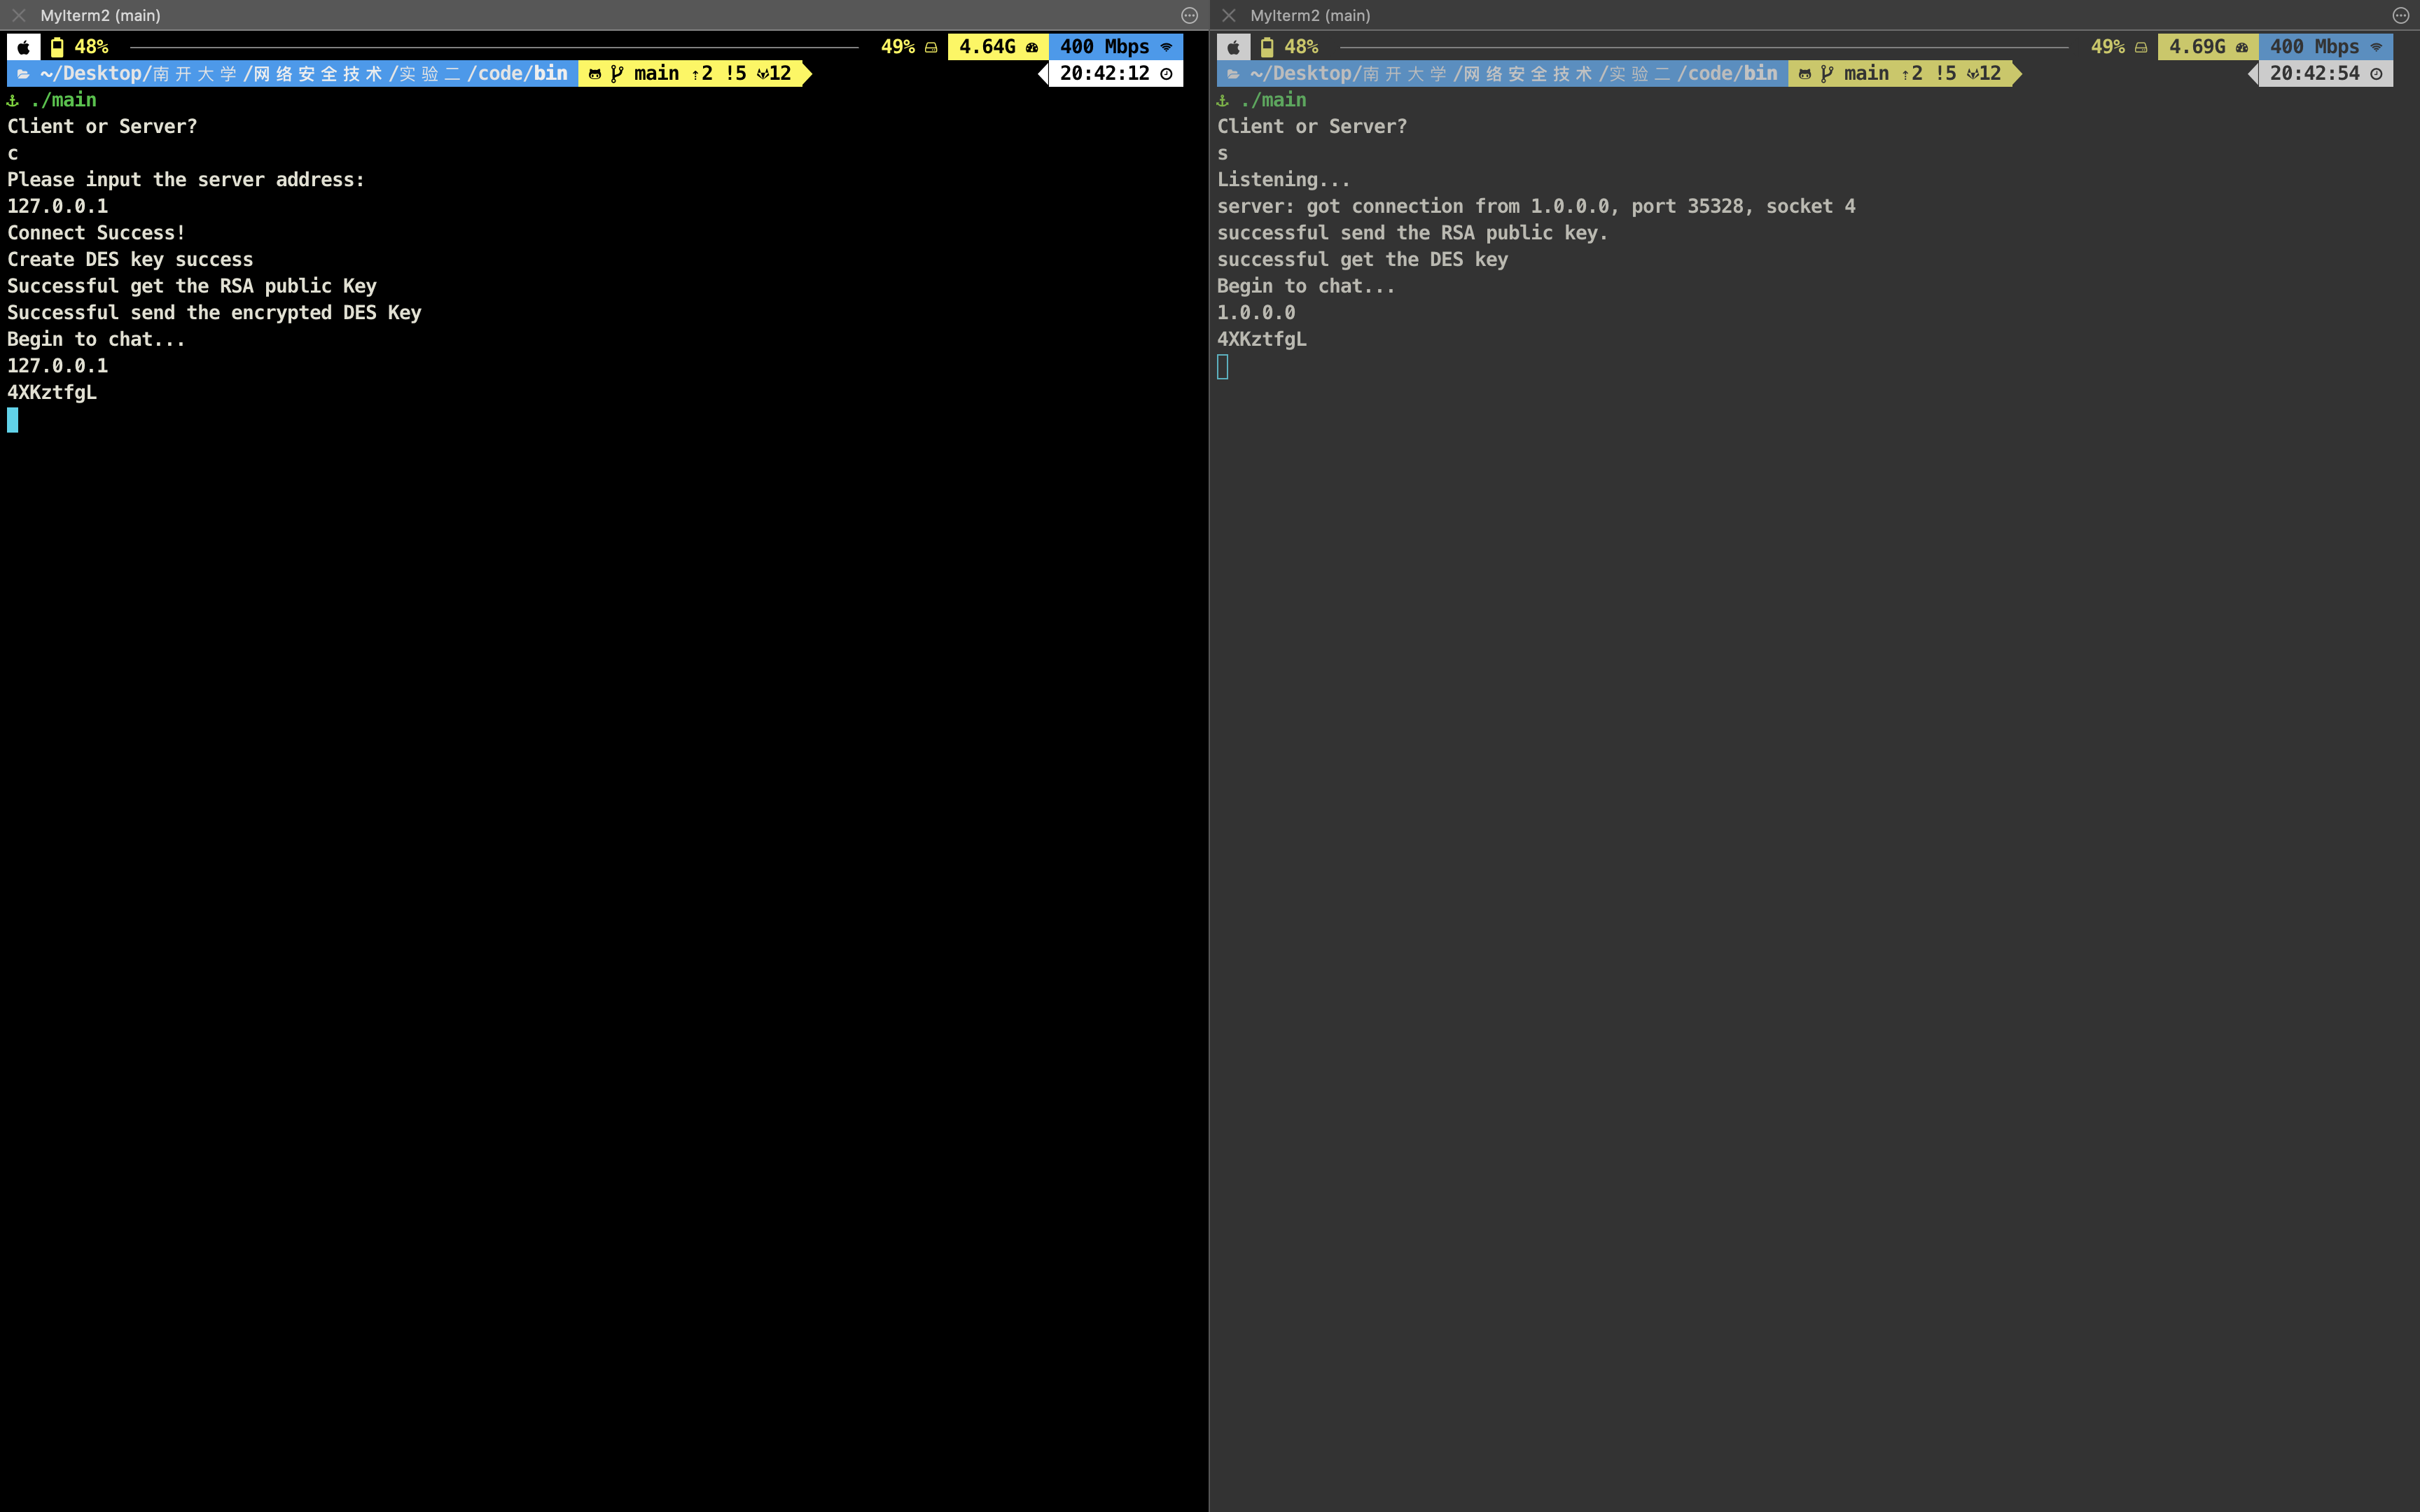
\includegraphics[scale = 0.23]{2.png}
\end{center}
客户端和服务端之间相互通信
\begin{center}
  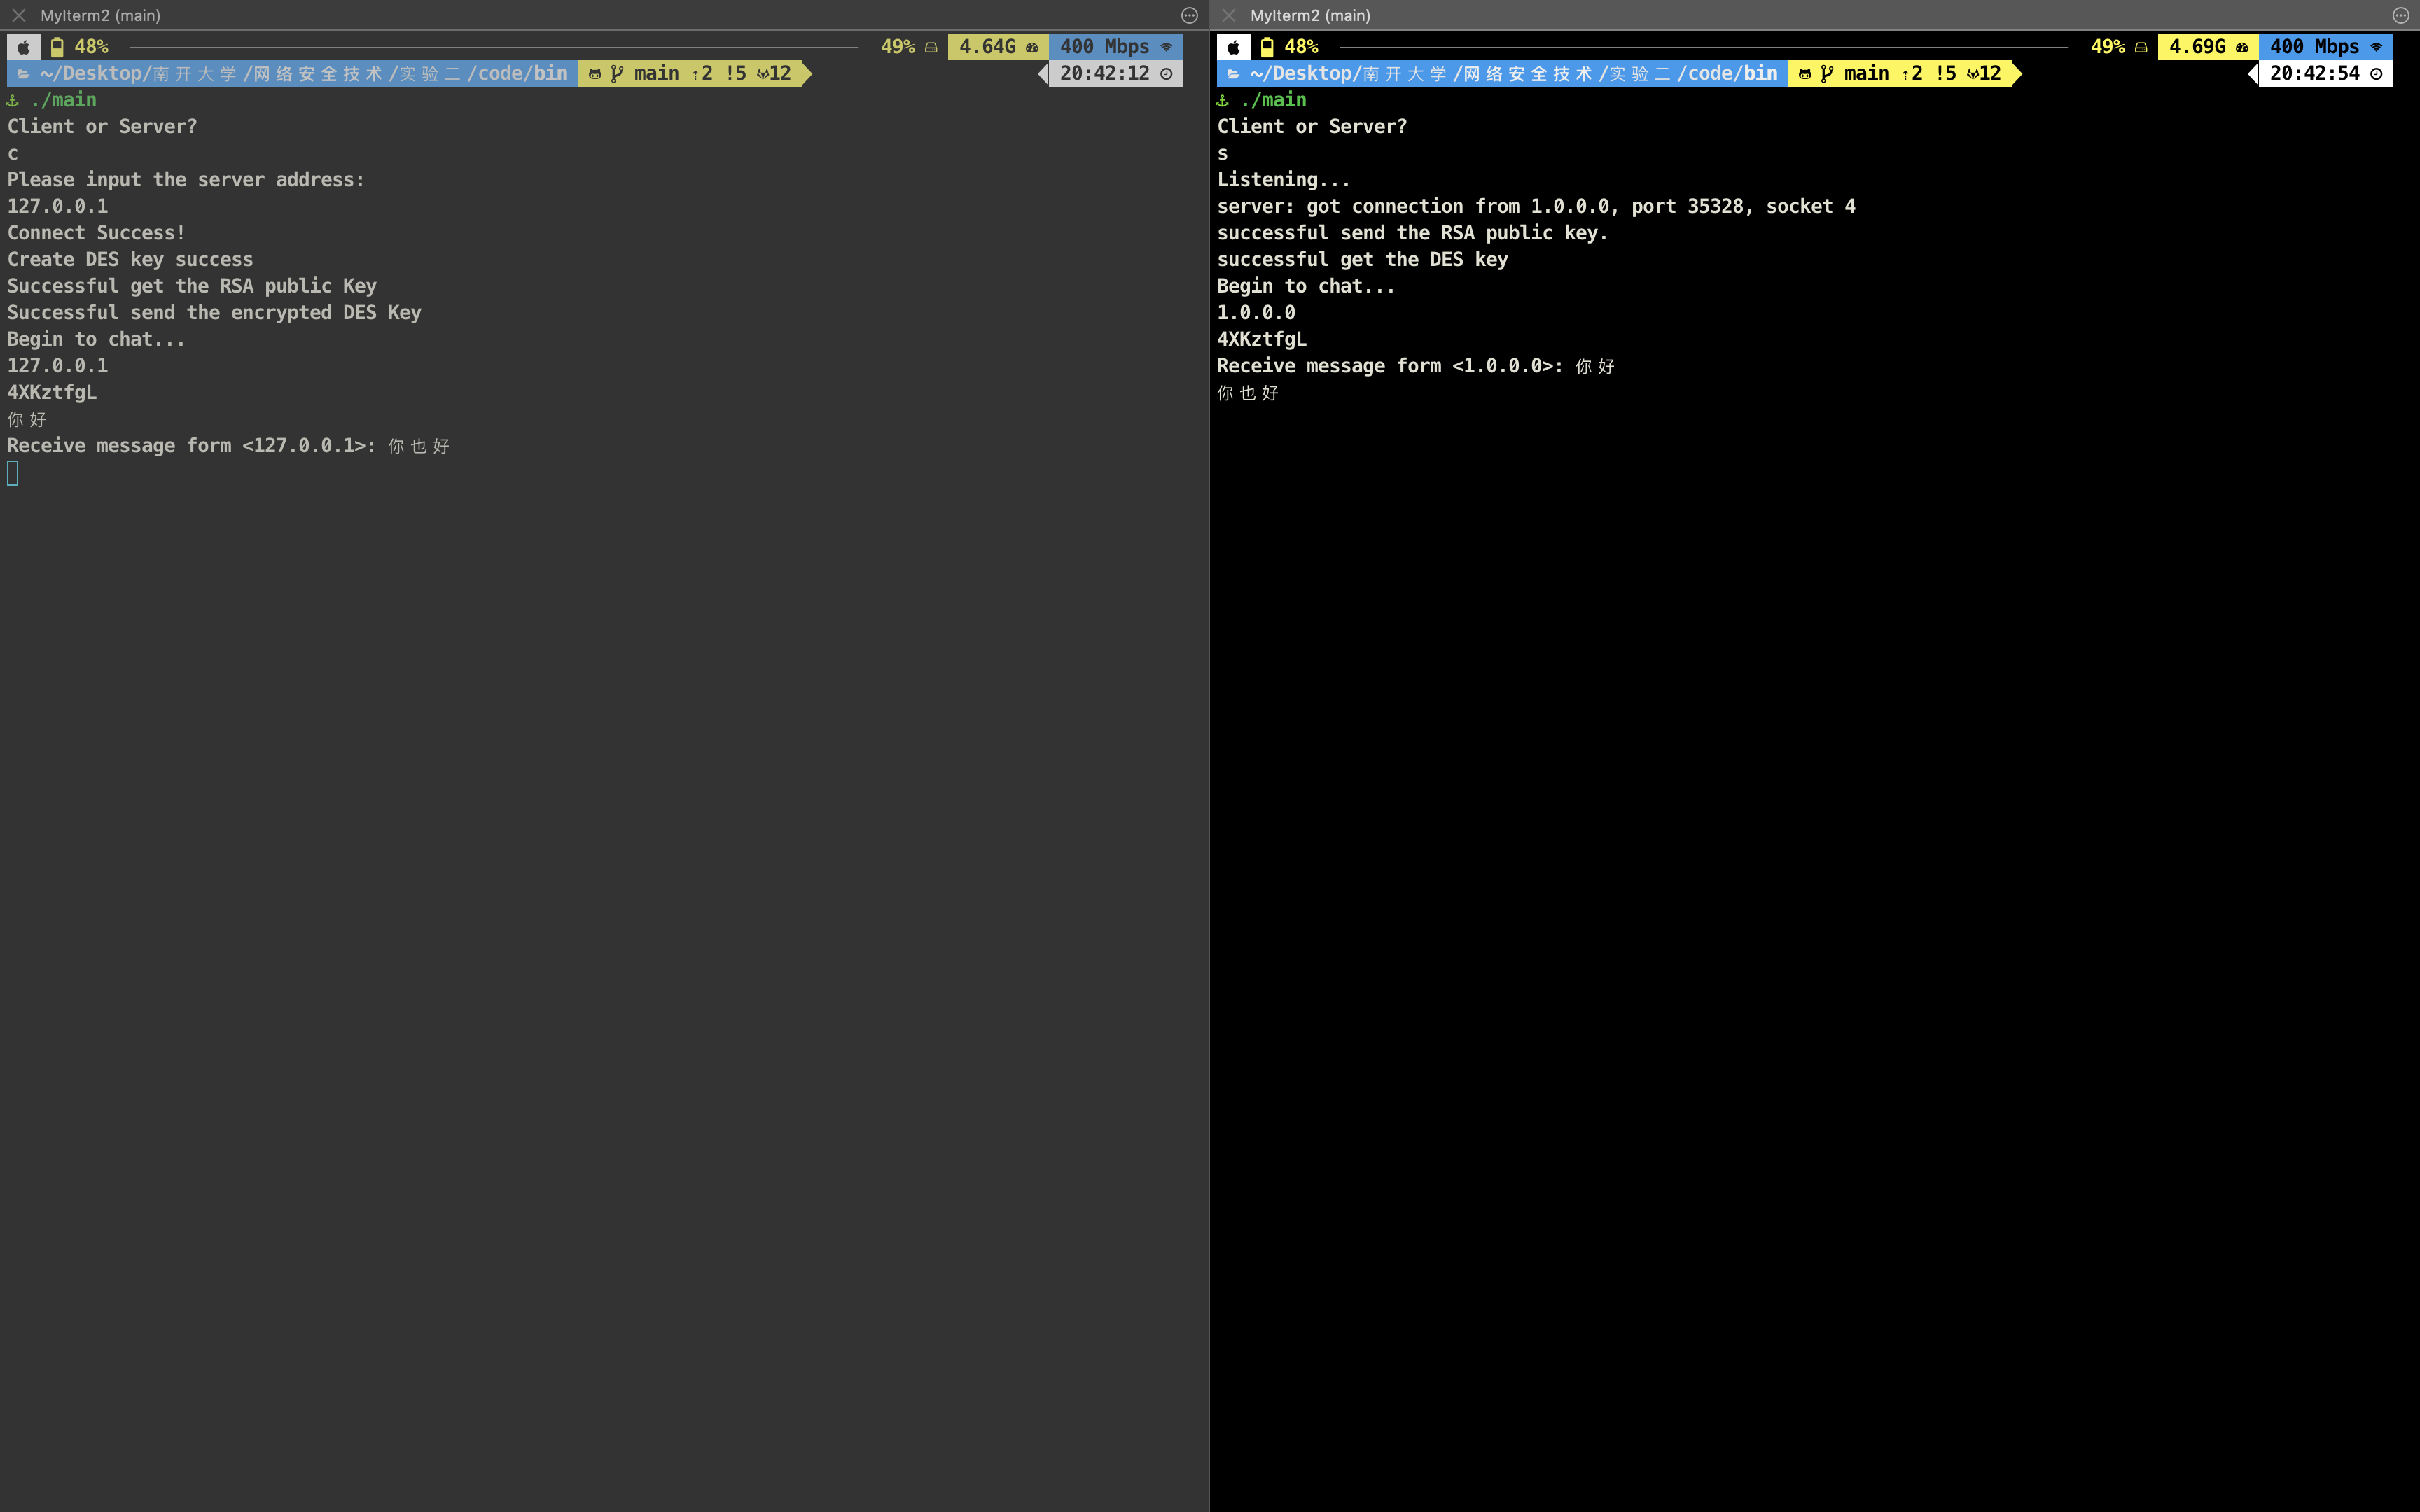
\includegraphics[scale = 0.23]{3.png}
\end{center}
输入Quit后停止通信
\begin{center}
  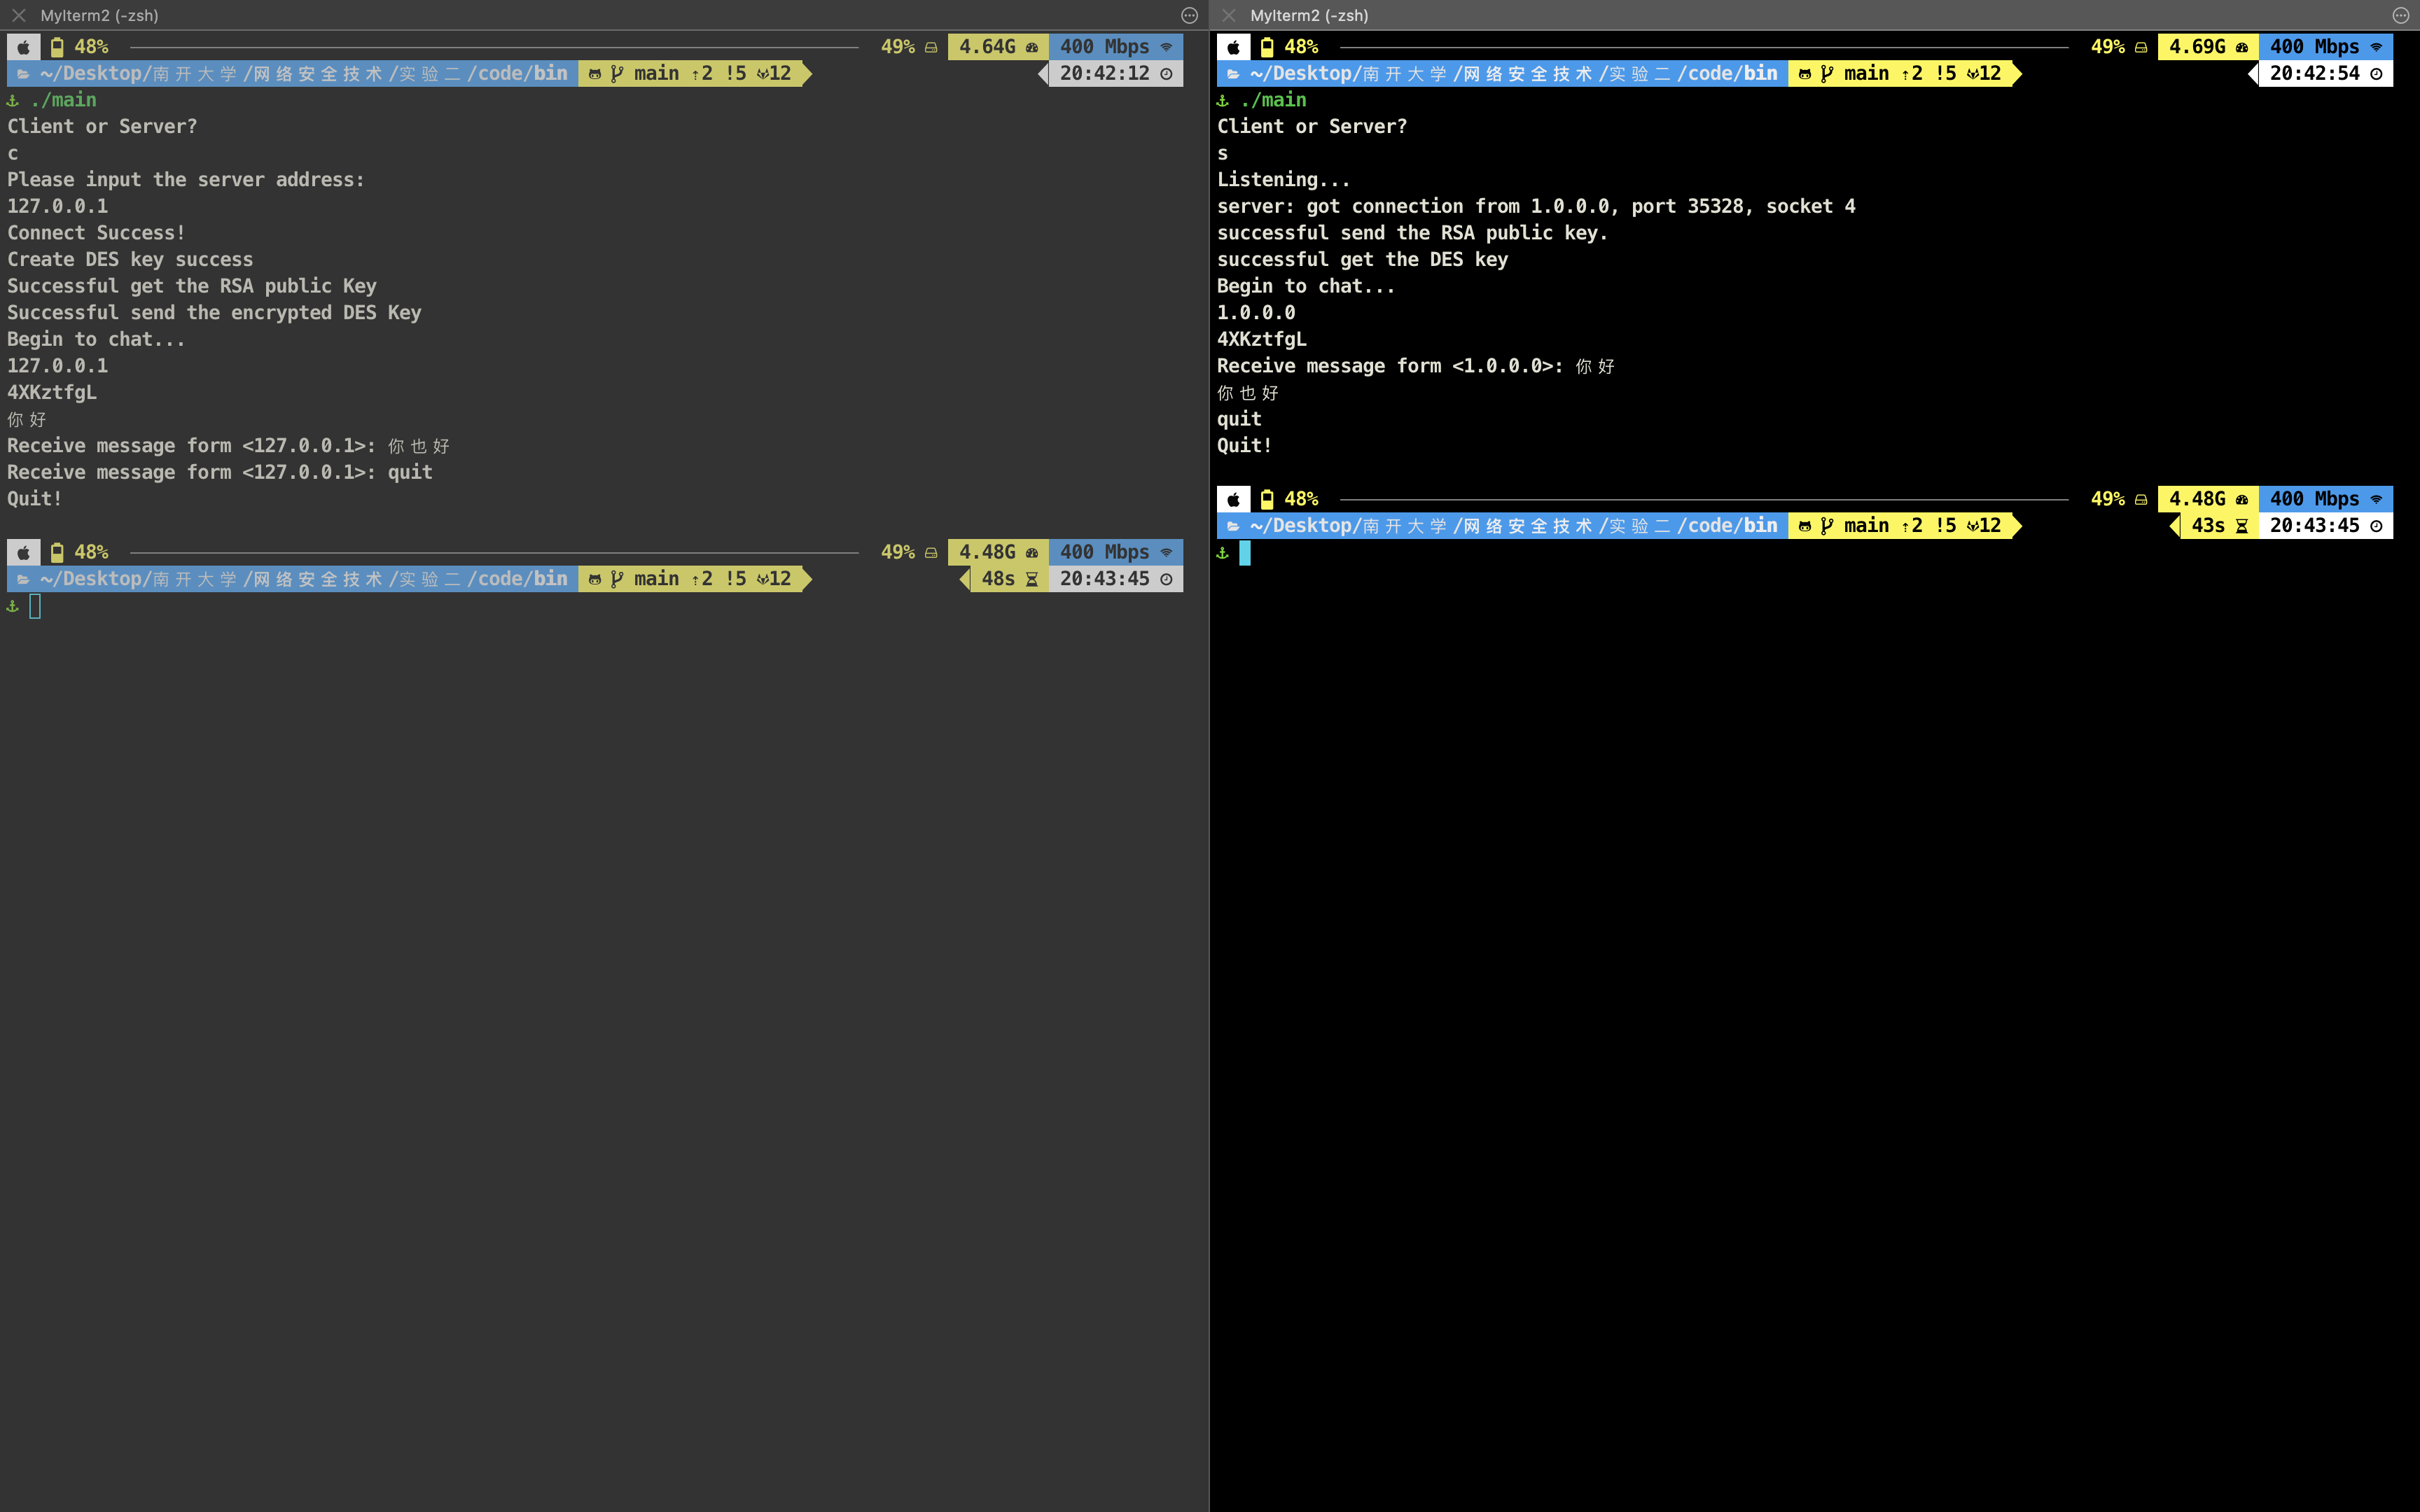
\includegraphics[scale = 0.23]{4.png}
\end{center}


\section{实验遇到的问题及其解决方法}
首先我们在使用Encry函数时,经历了如下报错
\begin{center}
  \includegraphics*[scale = 0.3]{截屏2022-04-07 00.34.42.png}
  \includegraphics*[scale = 0.5]{截屏2022-04-07 00.35.02.png}
\end{center}
可以看出,其问题在于,我们不能直接调用类的函数。为了解决这个问题,我们查阅了资料得知,应当在其前面加上static声明其为静态函数,便可以在类外直接调用。

然后是如何将整型(按ASCII 码值)转换成string 类型的问题。服务器接收到DES 的密文分别是四个短整型(2 个字大小)的值。如果使用to\_string 函数,则是将数字换成对应的字符串数字,如65 到“65”,并没有根据ASCII 码转换成对应的字符“A”。而如果仅仅在转换的短整型前面加上(char*)\&,则只能将短整型的第一个字节转换成字符,而少了一个。最终,我们使用使用sprintf 函数解决了这个转换的问题。


\section{实验结论}
本次实验在第一次实验,基于TCP的DES加密通讯的基础上实现了随机生成DES密钥、随机生成RSA公钥、密钥,并且通过RSA加密方法共享DES密钥。加深了对RSA 非对称加密算法的步骤的理解。本实验只使用了RSA 算法对
DES 密钥的传输进行加密解密,而不是完全使用RSA 加密解密,是因为RSA 算法执行的运算量比较大,系统消耗的资源会比较大。而只对DES 密钥共享进行RSA 加密,既保证了通信的安全,又节省了资源。此外值得注意的是,由于客户端加密DES 密钥时,只能获取RSA 的公钥对,而RSA类中的成员变量是公私钥对(对于客户端不可见),所以RSA 加密函数中的参数既包括了明文分组,又包括公钥对。

此外,我们较实验一的基础上,进一步掌握了Linux下的通信机制。使用select函数替换了了原来使用fork 进程的方法,减少了进程开销,在实现上也更加简单。

\end{document}